%\part*{Lezione 31/03/2021}
\section{Studio \textit{ab-initio}}\label{0331-sec-studioab}\index{Metodo ab-initio@Metodo \textit{ab-initio}}
La $pp$ non si riesce a misurare, tuttavia è possibile studiarla\footnote{Avvertiamo il lettore che ci saranno differenze di notazione rispetto a quando abbiamo mostrato il calcolo la prima volta.} col metodo che abbiamo discusso nella sezione \secrif{0318-sec-abinitio}; fu Bethe il primo a lavorarci, dando inizio al modello solare.\\
Prima di \vir{addentrarci} nel calcolo, osserviamo che la funzione d'onda finale sarà la stessa di quella per lo studio della reazione in sezione \secrif{0317-sec-abinitio}, poiché il prodotto di entrambe è un deutone, tuttavia si avranno differenze per le funzioni d'onda dei reagenti e per il fatto che la $pp$ non è mediata dall'interazione elettromagnetica.
$$p+p \to d+e^++\nu_e$$
Dunque studieremo la cinematica della reazione per avere la dipendenza dall'elemento di matrice ridotta e poi passeremo al calcolo di questo. 

\paragraph{Calcolo della cinematica.}Detto $w$ il \textit{rate} di decadimento, dalla teoria di Fermi\index{regola d'oro di Fermi}:
$$w = \frac{2\pi}{\hbar}|V_{fi}|^2\rho(E_f)$$
dove $V_{fi} = G_F M$ con $G_F$ costante di Fermi\index{costante di Fermi@costante di Fermi $G_F$}\index{costante di accoppiamento debole@costante di accoppiamento debole $g$} e $M$ elemento di matrice del decadimento $\beta^+$. Trascuriamo la massa del neutrino per cui $E_i-E_f\equiv E_0 = E_e + E_\nu = E + cq$ e nel centro di massa $\vec{p}_d = -\vec{p}-\vec{q}$ (non indipendente da $p$ e $q$, ma determinato da essi); possiamo allora riscrivere la densità di stati finali nello spazio delle fasi:
\begin{displaymath}
\begin{aligned}
dn &= \frac{d^3 p}{(2\pi\hbar)^3}\frac{d^3 q}{(2\pi\hbar)^3} =\\
&= \frac{p^2 q^2}{4\pi^4 \hbar^6} dpdq\: \footnotemark \\
\rho(E_f)\equiv \frac{dn}{dE_\nu} = \frac{dn}{cdq} &= \frac{p^2 (E_0-E)^2}{4\pi^4 c \hbar^6\,c^2} dp
\end{aligned}
\end{displaymath}
\footnotetext{Abbiamo integrato su $d\hat{q}d\hat{p}$.}
dove ci siamo limitati solo agli stati di interesse $dn/dE_\nu$ (come avevamo fatto nel decadimento $\beta$ fissando l'energia dell'elettrone e differenziando in $q$). Avremo quindi per il \textit{rate}:
$$dw = \frac{2\pi}{\hbar}|V_{fi}|^2\,\frac{p^2 (E_0-E)^2}{4\pi^4 c \hbar^6\,c^2} dp \stackrel{p\to E}{=} \frac{|V_{fi}|^2}{2\pi^3 \hbar^7 c^6} (E_0-E)^2 \sqrt{E^2 - m^2c^4} E dE $$
Ricordando che $d\sigma = dw/j_{inc} = dw/v$, integrando in $dE$ si ha\footnote{$c=\hbar=1$.}:
$$\sigma = \frac{1}{2\pi^3 v} G_F^2 |M|^2 \underbrace{\int_m^{E_0} (E_0-E)^2 \sqrt{E^2-m^2}E dE}_{\text{int. di Fermi } f(E_0)} $$\index{integrale di Fermi@integrale di Fermi $f(E_0)$}
$$|M|^2 \to \frac{1}{(2S_p +1)^2} \sum_{spin} |M|^2 = \frac{1}{4} \sum_{spin} |\int d^3x\: \psi^*_d (\vec{x})\,\psi_{pp}(\vec{x})|^2$$
dove abbiamo mediato sugli \textit{spin}\footnote{La parte di \textit{isospin} $\eta_d(\tau=0)(np)\sum_i\tau^-_i (pp)$ valutata sulle funzioni d'onda è 1.}. Da questo punto in poi adesso si procede numericamente, tuttavia a scopo illustrativo illustriamo il calcolo analitico che eseguì anche Bethe\footnote{L'articolo al quale ci riferiamo è Bethe, H. A. \& Critchfield, C. L., Phys. Rev., 1938, vol.54, p.248, \texttt{url:} \url{https://journals.aps.org/pr/abstract/10.1103/PhysRev.54.248}.\articolo{Bethe}}.

\paragraph{Risoluzione analitica.} Anche se il calcolo è analitico il risultato è piuttosto valido.\\
Per studiare $\psi_d$ prendiamo:
\begin{itemize}
    \item l'onda $S$ $\psi_d\to{^3S_1}$, per cui $\psi_d = u(r)/r$.
    \item buca di potenziale $V = -V_0$ per $r<r_0$.
    $$%
    \psi_d = \Bigl \{
    \begin{array}{llr}
        \frac{C}{r}\, e^{-\alpha r } & r>r_0 & \alpha\equiv \sqrt{mB}/\hbar \\
        \frac{C'}{r}\, \sin{(k_0 r)} & r<r_0 & k_0 \equiv \sqrt{m(V_0-B)}/\hbar
    \end{array}%
    $$
    Abbiamo allora $b\equiv 1/\alpha \simeq 4.4$ fm e definendo $x\equiv r/b$, $x_0\equiv r_0/b$ e $\mu \equiv \sqrt{(V_0-B)/B}=k_0/\alpha$ si ottiene:
    $$%
    \psi_d = \Bigl \{
    \begin{array}{ll}
        \frac{A}{r}\; e^{-(x-x_0)}\equiv \psi_> & r>r_0 \\
        \frac{A}{r}\; \sin{(\mu x)}/\sin{(\mu x_0)}\equiv \psi_< & r<r_0
    \end{array}%
    $$
    Osserviamo che questa espressione soddisfa automaticamente la continuità sia della funzione che della sua derivata in $r=r_0$, per cui dalla condizione di normalizzazione\footnote{$1=\int |\psi_d|^2=\int_0^{r_0}|\psi_<|^2+\int_{r_0}^\infty|\psi_>|^2$.} si ottiene\footnote{Successivamente per non confonderci con la costante che compare in $\psi_{pp}$ chiameremo questa $A\to A_d$.}:
    $$A = \frac{1}{\sqrt{2\pi b}}\, \frac{1}{\sqrt{1+x_0}}\,\frac{1}{\sqrt{1+\mu^{-2}}}$$
\end{itemize}
Studiamo a questo punto $\psi_{pp}$:
\begin{itemize}
    \item consideriamo sempre un'onda $S$ ($\ell=0$), perché le energie sono comunque basse\footnote{Si ricordi l'ordine di grandezza per le energie del picco di Gamow.}.
    \item prendiamo la stessa buca di potenziale, ma per $r>r_0$ consideriamo un potenziale coulombiano $V_{coul}$. Dovremo risolvere allora l'equazione di \Sch{} con $\psi_{pp} (r) = u(r)/r$:
    $$u'' - \frac{m}{\hbar^2} (V(r) - E)u =0$$
    Definita la massa ridotta $\mu\equiv m/2$ e $\rho\equiv kr$ con $k=\mu v /\hbar$ si ha\footnote{$E=\mu v^2/2 = \hbar^2 k^2/m$.} allora per $r<r_0$:
    $$\ppc{\frac{d^2}{d\rho^2} + 1 + \frac{2V_0}{\mu v^2}}u=0$$
    $$\psi_< (r) \: r = u(r) = A \, \sin{\ppc{\frac{\sqrt{mD}}{\hbar} r}} $$
    $$ D \equiv \underbrace{V_0}_{\sim\unit{MeV}} + \underbrace{\frac{\hbar^2k^2}{m}}_{\simeq 6\unit{keV}} \simeq V_0 $$
    Per quanto riguarda invece $r>r_0$ prendiamo le funzioni di Coulomb\footnote{Nel nostro caso $L=0$.}\index{funzioni di Coulomb} regolare $F_L(kr)$\index{funzioni di Coulomb!regolare} e irregolare $G_L(kr)$\index{funzioni di Coulomb!irregolare}:
    $$\psi_>(r) = \PPq{F_0 (kr) + \tan{(\delta_0)}\:G_0(kr)}\frac{e^{i\delta_0}\cos{(\delta_0)}}{kr}$$
    dove $\delta_0$ è lo sfasamento. Per trovare $A$ e $\delta_0$ imponiamo:
    \begin{itemize}
        \item continuità delle derivate logaritmiche:
        $$\frac{\psi_>'}{\psi_>}\Bigr |_{r=r_0} = \frac{\psi_<'}{\psi_<}\Bigr |_{r=r_0}$$
        $$\tan{\delta_0} = \frac{F_0(kr_0) - F_0(kr_0)\,\frac{d}{dr}\ln{w}(r_0)}{G_0(kr_0)\,\frac{d}{dr}\ln{w}(r_0) - G_0'(kr_0)}$$
        dove abbiamo definito $w(r) = A \sin{(\sqrt{mD}r/\hbar)}$.
        \item continuità delle funzioni in $r=r_0$:
        $$A \simeq \frac{F_0(kr_0)+\tan{\delta_0} G_0(kr_0)}{k\sin{(\sqrt{mD}r_0/\hbar)}}$$
        dove abbiamo approssimato $\cos{\delta_0}\sim e^{i\delta_0}\sim 1$ dal momento che $\delta_0\sim 0.002$.
    \end{itemize}
    Al tempo di Bethe $F_0$ e $G_0$ erano tabulate (non esistevano i calcolatori), per cui si aveva:
    $$F_0(kr)\simeq \underbrace{\sqrt{\frac{2\pi\gamma}{e^{2\pi\gamma}-1}}}_\text{Cost. Coulomb}kr\,\Phi(kr)\equiv C_0\, kr \, \Phi(kr) $$
    $$G_0(kr)=C_0^{-1} \, \Theta(kr)$$
    dove $\gamma \equiv Z_1Z_2e^2/\hbar v$ e $\Phi$ e $\Theta$ sono due polinomi tabulati\footnote{Non siamo interessati all'espressione di questi polinomi, ma la riportiamo solo per completezza:
    $$\Phi(kr)\simeq 1+\gamma\, kr - (2\gamma^2-1)\frac{(kr)^2}{6} + O((kr)^3) = \sum_{i=0}^\infty \varphi_i (kr)^i$$
    $$\Theta(kr) = \sum_{j=0}^\infty \theta_j (kr)^j + (2kr\gamma\ln{2kr}+f(\gamma))$$
    Basti ricordare che $\Phi$ è un polinomio \textit{smooth} e che $\Phi(0)=1$.\index{funzioni di Coulomb}}. Possiamo allora riscrivere:
    \begin{displaymath}
    \begin{aligned}
        &\tan{\delta_0} = C_0^2 \, kr_0 \, \lambda \\
        &A = C_0r_0\, \ppc{\frac{\Phi(kr_0)+\lambda\Theta(kr_0)}{\sin{(\nu \, r_0/b)}}}            
    \end{aligned}
    \end{displaymath}
    dove abbiamo raccolto\footnote{Questa è una notazione di Bethe} in $\lambda$ tutta la parte dipendente dai polinomi e abbiamo definito $b\equiv \hbar/\sqrt{mB}$ e $\nu\equiv \sqrt{mD} b/\hbar = \sqrt{D/B}$. Dunque, l'espressione di $\psi_{pp}$:
    \begin{displaymath}
        \begin{aligned}
            \psi_> &= C_0\, \PPq{\Phi(kr) + \lambda \frac{r_0}{r}\Theta(kr)}\\ 
            \psi_< &= \frac{C_0r_0}{r} \, \pp{[}{\Phi(kr_0)+\lambda\Theta(kr_0)}{]}\frac{\sin{(\nu r)/b}}{\sin{(\nu r_0)/b}}
        \end{aligned}
    \end{displaymath}
\end{itemize}
Possiamo adesso calcolare l'elemento di matrice\footnote{Si ricordi che $x\equiv r/b$.}:
%!
%%! C'è da capire che cos'è quella lambda e come si ottiene
%!
\begin{displaymath}
    \begin{aligned}
        M&=\int d^3x \: \psi^*_d(\vec{x}) \, \psi_{pp} (\vec{x}) = \\ 
        &= 4\pi \int_0^\infty r^2 dr \: \psi_d(r)\,\psi_{pp} (r)  = \\ 
        &=  4\pi \PPq{ \int_0^{r_0} r^2 dr \: \psi_{pp,<} (r)\, \psi_{d,<}(r) + \int_{r_0}^\infty r^2 dr \: \psi_{pp,>} (r)\, \psi_{d,>}(r) } \\ 
        &= 4\pi C_0 A_d b^2 \Bigl [ \frac{x_0}{\sin{\mu x_0}} \frac{(\Phi(kr_0)+\lambda\Theta(kr_0)}{\sin{\gamma x_0}} \int_0^{x_0} dx\, \sin{\mu x} \sin{\nu x} \\ 
        &+ \int_{x_0}^\infty dx\, xe^{-(x-x_0)}\Phi(kbx) + \lambda \int_{x_0}^\infty x_0 e^{-(x-x_0)}\Theta(kbx) \Bigr ] \equiv \\ 
        &\equiv 4\pi C_0 b^2 \, \frac{1}{\sqrt{2\pi b}}\, \frac{1}{\sqrt{1+x_0}}\,\frac{1}{\sqrt{1+\mu^{-2}}} \, \PPq{\Lambda_1+\Lambda_2+\Lambda_3} \equiv \\ 
        &\equiv 4\pi C_0b^2 \frac{1}{\sqrt{2\pi b}} \, \Lambda
    \end{aligned}
\end{displaymath}
dove abbiamo definito $\Lambda_i$ per raccogliere i vari integrali, anche se sono comunque tutti facilmente risolubili (prodotto di seni o integrali di polinomi per un esponenziale). Sostituiamo $M$ nell'espressione della sezione d'urto:
$$ \sigma = \frac{C_0^2 b^3}{\pi^2 v} G_F^2 f(E_0) \Lambda^2 $$

\subsection{Risultati}
Così facendo Bethe trovò $\Lambda^2 = 5.93 \div 8.08 $ e un fattore astrofisico\index{fattore astrofisico@fattore astrofisico $S(E)$} $S = ( 3.38 \div 4.61 )\cdot\ord{-25}$ MeVb. I risultati\footnote{\acc{E} interessante osservare che il neutrino fu teorizzato proprio nel 1938 e Bethe ne tiene di conto, tuttavia non lo riporta.} globali sono riportati in Tabella \ref{0331_tab}.
\begin{figure}[h]
    \centering
    \includegraphics*[scale=0.5]{Immagini/0331_Bethetab.png}
    \caption{Risultati di Bethe per $r_0 \simeq  3$ fm e $r_0 \simeq 1.5$ fm.}
    \label{0331_tab}
\end{figure}
\newline
\noindent L'\vir{enorme} incertezza sul fattore astrofisico della $pp$ si ripercuote anche sulle successive stime del flusso di neutrini solari, per questa ragione nel 1998 fu fatto un altro calcolo con potenziali dipendenti dal tempo (AV18\index{potenziali realistici@potenziali \textit{realistici}!AV18} e CD-Bonn\index{potenziali realistici@potenziali \textit{realistici}!CD-Bonn}) detti \textit{realistici} perché riproducono tutti i dati sperimentali $NN + d$ con un rapporto $\chi^2/\text{dati}\sim 1.04$.
%!
%%! Che si intende con questo NN + d:
%%! forse sta per Nucleone-Nucleone o Nucleo-Nucleo?
%!
Inoltre in questo studio non è stato considerato solo l'operatore di \textit{isospin}, ma un operatore di Gamow-Teller\index{operatore di Gamow-Teller}\index{decadimento di!Gamow-Teller}, quindi a un corpo, perché si ha infatti il passaggio ${^1S_0} \to {^3S_1}$, ovvero un operatore vettoriale nello spazio dello \textit{spin} $\sum_i \vec{\sigma}_i \tau^\pm_i$. Per questo operatore è possibile fare uno studio \textit{ab-initio} sui decadimenti $\beta$\index{decadimento $\beta$} di nuclei leggeri come $\ce{^3H}\to\ce{^3He} +e^- + \bar{\nu}_e$: utilizzando tale operatore a un corpo sottostimiamo\footnote{Esiste tuttavia un parametro nella teoria della MEC per correggere tale sottostima.} $\tau_{1/2}$ di circa il 4\% e questo è dovuto al fatto di aver trascurato le \textit{meson-exchange currents}\index{meson-exchange current@$J_{ij}^{MEC}$ \textit{meson-exchange current}}.
\begin{figure}[h]
    \centering
    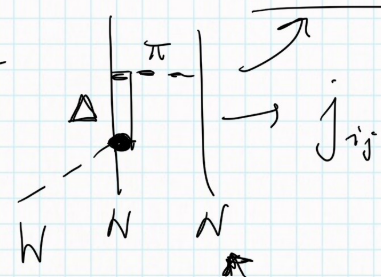
\includegraphics[scale=0.5]{Immagini/0331_GT.png}
    \caption{Schema del decadimento $\beta$ con nuclei leggeri. $N$ sono i nuclei, $W$ è il bosone di interazione, $\pi$ è la corrente di mesoni e $\Delta$ è la risonanza che si diseccita.}%! Capisci meglio
    \label{0331_MEC}
\end{figure}
\newline
\noindent Tornando al lavoro del 1998, che tenne conto del parametro di correzione all'operatore GT, si ottenne $\Lambda^2 = 7.035$ (circa il valore centrale del \textit{range} trovato da Bethe) e un fattore astrofisico $S(0) = 4.01 (1.000\pm0.009)\cdot\ord{-25}$ MeVb. Nel 2008 il conto è stato rifatto, ma con una trattazione dell'errore più rigorosa ed è stato confermato il risultato.
